\begin{task}
\TT{Wyznacz współczynniki zespolonego szeregu Fouriera dla okresowego sygnału $g(t)$ przedstawionego na rysunku. Wykorzystaj własności szeregu Fouriera oraz współczynniki zespolonego szeregu Fouriera wyznaczone w zadaniu \ref{TaskKW012}}{Calculate coefficients of the periodic signal $f(t)$ shown below for the expansion into a complex exponential Fourier series. Draw magnitude and phase spectra.}

\begin{figure}[H]
\centering
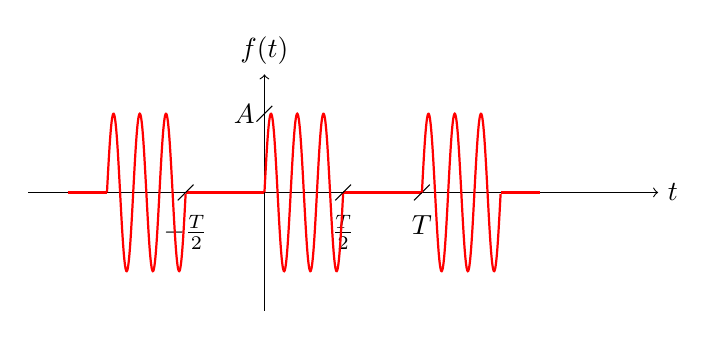
\begin{tikzpicture}
  %\draw (0,0) circle (1in);
  \draw[->] (-3.0,+0.0) -- (+5.0,+0.0) node[right] {$t$};
  \draw[->] (+0.0,-1.5) -- (+0.0,+1.5) node[above] {$f(t)$};
  \draw[-,red, thick] (-2.5,+0.0) -- (-2.0,+0.0);
  \draw[-,red, thick] (-1.0,+0.0) -- (+0.0,+0.0);
  \draw[-,red, thick] (+1.0,+0.0) -- (+2.0,+0.0);
  \draw[-,red, thick] (+3.0,+0.0) -- (+3.5,+0.0);
  %\draw[-] (-1.0-0.1,-0.1)--(-1.0+0.1,0.1) node[midway, below, outer sep=10pt,align=center] {$-\frac{T}{2}$};
  \draw[-] (-1.0-0.1,-0.1)--(-1.0+0.1,0.1) node[midway, below, outer sep=5pt,align=center] {$-\frac{T}{2}$};
  \draw[-] (+1.0-0.1,-0.1)--(+1.0+0.1,0.1) node[midway, below, outer sep=5pt] {$\frac{T}{2}$};
  \draw[-] (+2.0-0.1,-0.1)--(+2.0+0.1,0.1) node[midway, below, outer sep=5pt] {$T$};
  \draw[-] (-0.1,1.0-0.1)--(+0.1,1.0+0.1) node[midway, left] {$A$};
  
  \draw[scale=1.0,domain=0:1.0,samples=200,smooth,variable=\x,red,thick] plot ({\x},{0.0+1.0*sin(\x*180.0/3.141592*6*3.141592/1.0)});
  \draw[scale=1.0,domain=2.0:3.0,samples=200,smooth,variable=\x,red,thick] plot ({\x},{0.0+1.0*sin(\x*180.0/3.141592*6*3.141592/1.0)});
  \draw[scale=1.0,domain=-2.0:-1.0,samples=200,smooth,variable=\x,red,thick] plot ({\x},{0.0+1.0*sin(\x*180.0/3.141592*6*3.141592/1.0)});
\end{tikzpicture}
\end{figure}

\TT{W pierwszej kolejności należy opisać sygnał za pomocą wzoru.}{Periodic signal $f(t)$, as a piecewise linear function, is given by:}

\begin{equation}
   f(x)=\begin{cases}A\cdot sin\left(\frac{12\pi}{T}\cdot t\right) & t \in \left (  0+k \cdot T; \frac{T}{2}+k \cdot T \right ) \\0 & t \in \left ( \frac{T}{2}+k \cdot T; T +k \cdot T\right )\end{cases} \wedge k \in \TT{C}{Z}
\end{equation}

\TT{Można zauważyć iż sygnał $g(t)$ jest z modulowaną wersją sygnału $f(t)$ z zadania \ref{TaskKW012}}{}
\begin{align*}
g(t) &= f\left(t\right) \cdot sin\left(\frac{12\pi}{T}\cdot t\right) \\
&=\left\{\begin{array}{ll}
\EulerSin
\end{array}\right\}=\\
&= f\left(t\right) \cdot \frac{e^{\jmath \cdot \frac{12\pi}{T}\cdot t} - e^{-\jmath \cdot \frac{12\pi}{T}\cdot t}}{2 \cdot \jmath} \\
&= \frac{1}{2\cdot \jmath} \left( f\left(t\right) \cdot e^{\jmath \cdot \frac{12\pi}{T}\cdot t} - f\left(t\right) \cdot e^{-\jmath \cdot \frac{12\pi}{T}\cdot t}\right)
\end{align*}

\TT{Współczynniki zespolonego szeregu Fouriera $F_k$ dla sygnału $f(t)$ wyznaczone w zadaniu \ref{TaskKW012} wynoszą:}{}
\begin{align*}
F_0&=\frac{A}{2}\\
F_k&=\jmath \cdot \frac{A}{k\cdot 2 \pi}\cdot \left( (-1)^{k} -1 \right)\\
\end{align*}

\TT{Korzystając z twierdzenia o modulacji można wyznaczyć współczynniki $G_k$ na podstawie współczynników $F_k$ sygnału $f(t)$ jako:}{}
\begin{align*}
g^1(t) &= f(t)\cdot e^{\jmath \cdot \frac{2\pi}{T}\cdot k_0 \cdot t}\\
G^1_k &= F_{k-k_0}
\end{align*}

\TT{W przypadku analizowanego sygnału twierdzenie o modulacji należy zastosować dwa razy}{}

\begin{align*}
g(t) &= \frac{1}{2\cdot \jmath} f(t)\cdot e^{\jmath \cdot \frac{2\pi}{T}\cdot k^1_0 \cdot t} - \frac{1}{2\cdot \jmath} f(t)\cdot e^{\jmath \cdot \frac{2\pi}{T}\cdot k^2_0 \cdot t}\\
g(t) & = g^1(t) - g^2(t)\\
G_k &= G^1_k - G^2_k\\
G_k &= \frac{1}{2\cdot \jmath} \left( F_{k-k^1_0} - F_{k-k^2_0} \right)
\end{align*}
  
\TT{W obu przypadkach funkcja $f(t)$ mnożona jest przez czynnik $e^{\jmath \cdot \frac{12\pi}{T}\cdot t}$ (z uwzględnieniem zmiany znaku). Z tego czynnika można wydzielić wartość $k^1_0$ i $k^2_0$.}{}

\begin{align*}
e^{\jmath \cdot \frac{12\pi}{T}\cdot t} &= e^{\jmath \cdot \frac{2 \ cdot 6\pi}{T}\cdot t}\\
&=e^{\jmath \cdot \frac{2\pi}{T} \cdot 6\cdot t} \Rightarrow k^1_0 = 6\\
\end{align*}

\begin{align*}
e^{-\jmath \cdot \frac{12\pi}{T}\cdot t} &= e^{-\jmath \cdot \frac{2 \ cdot 6\pi}{T}\cdot t}\\
&=e^{-\jmath \cdot \frac{2\pi}{T} \cdot 6\cdot t} \\
&=e^{\jmath \cdot \frac{2\pi}{T} \cdot \left(-6\right) \cdot t} \Rightarrow k^2_0 = -6\\
\end{align*}
  
\TT{Wstawiając wartości współczynników $F_k$ otrzymujemy}{}
\begin{align*}
G_k &= \frac{1}{2\cdot \jmath} \left( F_{k-k^1_0} - F_{k-k^2_0} \right) =\\
 &= \frac{1}{2\cdot \jmath} \left( 
\jmath \cdot \frac{A}{\left(k-k^1_0\right)\cdot 2 \pi}\cdot \left( (-1)^{k-k^1_0} -1 \right)
 - \jmath \cdot \frac{A}{\left(k-k^2_0\right)\cdot 2 \pi}\cdot \left( (-1)^{k-k^2_0} -1 \right) \right) = \\
&=\left\{\begin{array}{ll}
k^1_0 = 6 & k^2_0 = -6
\end{array}\right\}=\\ 
&= \frac{1}{2\cdot \jmath} \left( 
\jmath \cdot \frac{A}{\left(k-6\right)\cdot 2 \pi}\cdot \left( (-1)^{k-6} -1 \right)
- \jmath \cdot \frac{A}{\left(k-\left(-6\right)\right)\cdot 2 \pi}\cdot \left( (-1)^{k-\left(-6\right)} -1 \right) \right) =\\
&= \frac{1}{2\cdot \jmath} \left( 
\jmath \cdot \frac{A}{\left(k-6\right)\cdot 2 \pi}\cdot \left( (-1)^{k-6} -1 \right)
- \jmath \cdot \frac{A}{\left(k+6\right)\cdot 2 \pi}\cdot \left( (-1)^{k+6} -1 \right) \right) =\\
&= \frac{1}{2\cdot \jmath} \left( 
\jmath \cdot \frac{A}{\left(k-6\right)\cdot 2 \pi}\cdot \left( (-1)^{k} \cdot (-1)^{-6} -1 \right)
- \jmath \cdot \frac{A}{\left(k+6\right)\cdot 2 \pi}\cdot \left( (-1)^{k} \cdot (-1)^{6} -1 \right) \right) =\\
&= \frac{1}{2\cdot \jmath} \left( 
\jmath \cdot \frac{A}{\left(k-6\right)\cdot 2 \pi}\cdot \left( (-1)^{k} \cdot 1 -1 \right)
- \jmath \cdot \frac{A}{\left(k+6\right)\cdot 2 \pi}\cdot \left( (-1)^{k} \cdot 1 -1 \right) \right) =\\
&= \frac{1}{2\cdot \jmath} \left( 
\jmath \cdot \frac{A}{\left(k-6\right)\cdot 2 \pi}\cdot \left( (-1)^{k} -1 \right)
- \jmath \cdot \frac{A}{\left(k+6\right)\cdot 2 \pi}\cdot \left( (-1)^{k} -1 \right) \right) =\\
&= \frac{1}{2\cdot \jmath} \left( 
\jmath \cdot \frac{A}{\left(k-6\right)\cdot 2 \pi}
- \jmath \cdot \frac{A}{\left(k+6\right)\cdot 2 \pi}\right) \cdot \left( (-1)^{k} -1 \right) =\\
&= \frac{1}{2\cdot \jmath} \cdot \jmath \cdot \frac{A}{2\pi}\left( 
\frac{1}{k-6}
- \frac{1}{k+6}\right) \cdot \left( (-1)^{k} -1 \right) =\\
&= \frac{A}{4\pi}\left( \frac{k+6}{\left(k-6\right)\cdot \left(k+6\right)} - \frac{k-6}{\left(k-6\right)\cdot \left(k+6\right)}\right) \cdot \left( (-1)^{k} -1 \right) =\\
&= \frac{A}{4\pi}\left( \frac{k+6 - k +6}{\left(k-6\right)\cdot \left(k+6\right)} \right) \cdot \left( (-1)^{k} -1 \right) =\\
&= \frac{A}{4\pi}\left( \frac{12}{k^2-36} \right) \cdot \left( (-1)^{k} -1 \right) =\\
&= \frac{A}{\pi}\left( \frac{3}{k^2-36} \right) \cdot \left( (-1)^{k} -1 \right) =\\
&= \frac{3 \cdot A}{\pi \cdot \left( k^2-36 \right)} \cdot \left( (-1)^{k} -1 \right)
\end{align*}

\TT{A wiec współczynniki $G_k$ dla sygnału $g(t)$ są równe $\frac{3 \cdot A}{\pi \cdot \left( k^2-36 \right)} \cdot \left( (-1)^{k} -1 \right)$, dla $k \neq 6 \wedge k\neq -6$. Oznacza to iż współczynnik dla $k=6$ i $k=-6$ musimy wyznaczyć jeszcze raz analizując dokładnie co podstawiamy. Zacznijmy od wyznaczenia $G_6$ }{}

\begin{align*}
G_6 &= \frac{1}{2\cdot \jmath} \left( F_{6-k^1_0} - F_{6-k^2_0} \right) = \\
&=\left\{\begin{array}{ll}
k^1_0 = 6 & k^2_0 = -6
\end{array}\right\}=\\ 
&= \frac{1}{2\cdot \jmath} \left( F_{6-6} - F_{6-\left(-6\right)} \right) =\\
&= \frac{1}{2\cdot \jmath} \left( F_{0} - F_{6+6} \right) =\\
&= \frac{1}{2\cdot \jmath} \left( F_{0} - F_{12} \right)
\end{align*}

\TT{A wiec musimy podstawić wartość współczynników $F_0$ oraz $F_{12}$}{}

\begin{align*}
G_6 &= \frac{1}{2\cdot \jmath} \left( F_{0} - F_{12)} \right) =\\
&= \frac{1}{2\cdot \jmath} \left(\frac{A}{2} - \jmath \cdot \frac{A}{12\cdot 2 \pi}\cdot \left( (-1)^{12} -1 \right)\right) = \\
&= \frac{1}{2\cdot \jmath} \cdot \frac{A}{2} - \frac{1}{2\cdot \jmath} \cdot \jmath \cdot \frac{A}{12\cdot 2 \pi}\cdot \left( (-1)^{12} -1 \right) = \\
&= \frac{A}{4\cdot \jmath} - \frac{A}{12\cdot 4 \pi}\cdot \left( 1 -1 \right) = \\
&= \frac{A}{4\cdot \jmath} - \frac{A}{12\cdot 4 \pi}\cdot \left(0 \right) = \\
&= \frac{A}{4\cdot \jmath} - \frac{A}{12\cdot 4 \pi}\cdot 0 = \\
&= \frac{A}{4\cdot \jmath} -  0 = \\
&= \frac{A}{4\cdot \jmath}
\end{align*}


\TT{Podobnie wyznaczymy współczynnik $G_{-6}$ }{}

\begin{align*}
G_{-6} &= \frac{1}{2\cdot \jmath} \left( F_{-6-k^1_0} - F_{-6-k^2_0} \right) = \\
&=\left\{\begin{array}{ll}
k^1_0 = 6 & k^2_0 = -6
\end{array}\right\}=\\ 
&= \frac{1}{2\cdot \jmath} \left( F_{-6-6} - F_{-6-\left(-6\right)} \right) =\\
&= \frac{1}{2\cdot \jmath} \left( F_{-12} - F_{-6+6} \right) =\\
&= \frac{1}{2\cdot \jmath} \left( F_{-12} - F_{0} \right)
\end{align*}

\TT{A wiec musimy podstawić wartość współczynników $F_{-12}$ oraz $F_{0}$}{}

\begin{align*}
G_6 &= \frac{1}{2\cdot \jmath} \left( F_{-12} - F_{0)} \right) =\\
&= \frac{1}{2\cdot \jmath} \left( \jmath \cdot \frac{A}{-12\cdot 2 \pi}\cdot \left( (-1)^{-12} -1 \right) - \frac{A}{2}\right) = \\
&= \frac{1}{2\cdot \jmath} \left( \jmath \cdot \frac{A}{12\cdot 2 \pi}\cdot \left( 1 -1 \right) - \frac{A}{2}\right) = \\
&= \frac{1}{2\cdot \jmath} \left( \jmath \cdot \frac{A}{12\cdot 2 \pi}\cdot \left( 0 \right) - \frac{A}{2}\right) = \\
&= \frac{1}{2\cdot \jmath} \left( 0 - \frac{A}{2}\right) = \\
&= \frac{1}{2\cdot \jmath} \left( - \frac{A}{2}\right) = \\
&= -\frac{1}{2\cdot \jmath} \cdot \frac{A}{2} = \\
&= -\frac{A}{4\cdot \jmath}
\end{align*}

\TT{Można także zauważyć iż nie ma konieczności wyznaczania osobno wartości współczynnika dla $k=0$, ponieważ można go wyznaczyć z ogólnego wzoru na $G_k$.}{}


\TT{Ostatecznie współczynniki zespolonego szeregu Fouriera dla funkcji przedstawionej na rysunku przyjmują wartości.}{To sum up, coefficients for the expansion into a complex exponential Fourier series are given by:}
\begin{align*}
G_{-6}&=-\frac{A}{4\cdot \jmath}\\
G_{6}&=\frac{A}{4\cdot \jmath}\\
G_k&=\frac{3 \cdot A}{\pi \cdot \left( k^2-36 \right)} \cdot \left( (-1)^{k} -1 \right)
\end{align*}

\end{task}